
\section{GRAGPoison}
\label{sec:GRAGPoison}

Next, we introduce \attack, a novel attack designed specifically for \rag that addresses key limitations of existing attacks. Our attack innovates in two ways: it achieves higher effectiveness by poisoning relations rather than answers to exploit \rag's graph-based retrieval, and it improves scalability by generating poisoning text that compromises multiple queries simultaneously.

As illustrated in Figure~\ref{framework}, \attack operates in three phases: \mct{i} relation selection (\msec{Related Query Recognition}) -- it employs an LLM to extract and identify critical relations shared across target queries; \mct{ii} relation injection (\msec{Relation Replacement Attack}) -- it generates poisoning text to inject competing relations that substitute the selected shared relations; \mct{iii} relation enhancement (\msec{Relation Enhancement Attack}) -- it generates additional poisoning text to create supporting relations that strengthen the injected relations and ensure their retrieval by \rag.




\subsection{Relation Selection}
\label{Related Query Recognition}
For a given set of target queries $X$, \attack first identifies the entities and relations involved in $X$.

In the simple setting that the adversary is aware of the underlying knowledge graph, it is trivial to match each query $x \in X$ to a subgraph in the knowledge graph and explicitly identify relations shared across queries. We focus on the setting that given target queries set $X$, the adversary must deduce the underlying subgraph corresponding to each $x \in X$ without direct knowledge graph access. To achieve this, \attack exploits the adversarial LLM's chain-of-thought (CoT) reasoning capability. With careful prompting (details in \msec{sec:prompt_agnostic}), the LLM breaks down each multi-hop query into step-by-step reasoning\mcite{weiChainofThoughtPromptingElicits2022} and infers intermediate entities and relations. Further, the LLM identifies shared relations across queries by aggregating these intermediates, accounting for different references to the same entities and relations.

\begin{mtbox}{}
\begin{example} 
\label{exp:cot}
Given queries \msf{How to mitigate the malware Stuxnet?} and \msf{How to detect the malware Stuxnet?}, \attack deduces their query subgraphs and identifies a shared relation: \msf{Stuxnet uses \{a kind of attack method\}}. Note that the attack method entity remains unspecified at this stage.
\end{example}
\end{mtbox}

Formally, for each query $x \in X$, \attack identifies $V_x$ and $R_x$ as entities and relations involved in $x$. To minimize the amount of poisoning text, \attack strategically selects and poisons a subset of relations shared across multiple queries. We define that relation $r$ ``covers'' query $x$ if $r \in R_x$. This formulation reduces to the classical set cover problem\mcite{set-cover}. To identify an (approximately) minimal subset of relations, \attack employs a greedy algorithm as sketched in Algorithm~\ref{alg:query-selection}, which iteratively selects the relation that covers the maximum number of previously uncovered queries, achieving the best possible polynomial-time approximation of the optimal subset.

\begin{algorithm}\small 
\KwIn{$X$: target queries}
\KwOut{$R$: target relations}
$R \leftarrow \emptyset$\;
\While{$X$ are not fully covered}{
select $r \in  \cup_{x \in X}R_x$ that maximally covers queries in $X$\;
add $r$ to $R$\;
remove covered queries from $X$\;
}
\Return $R$\;
\caption{Selection of target relations. \label{alg:query-selection}}
\end{algorithm}





\begin{figure*}[!ht]
\centering
    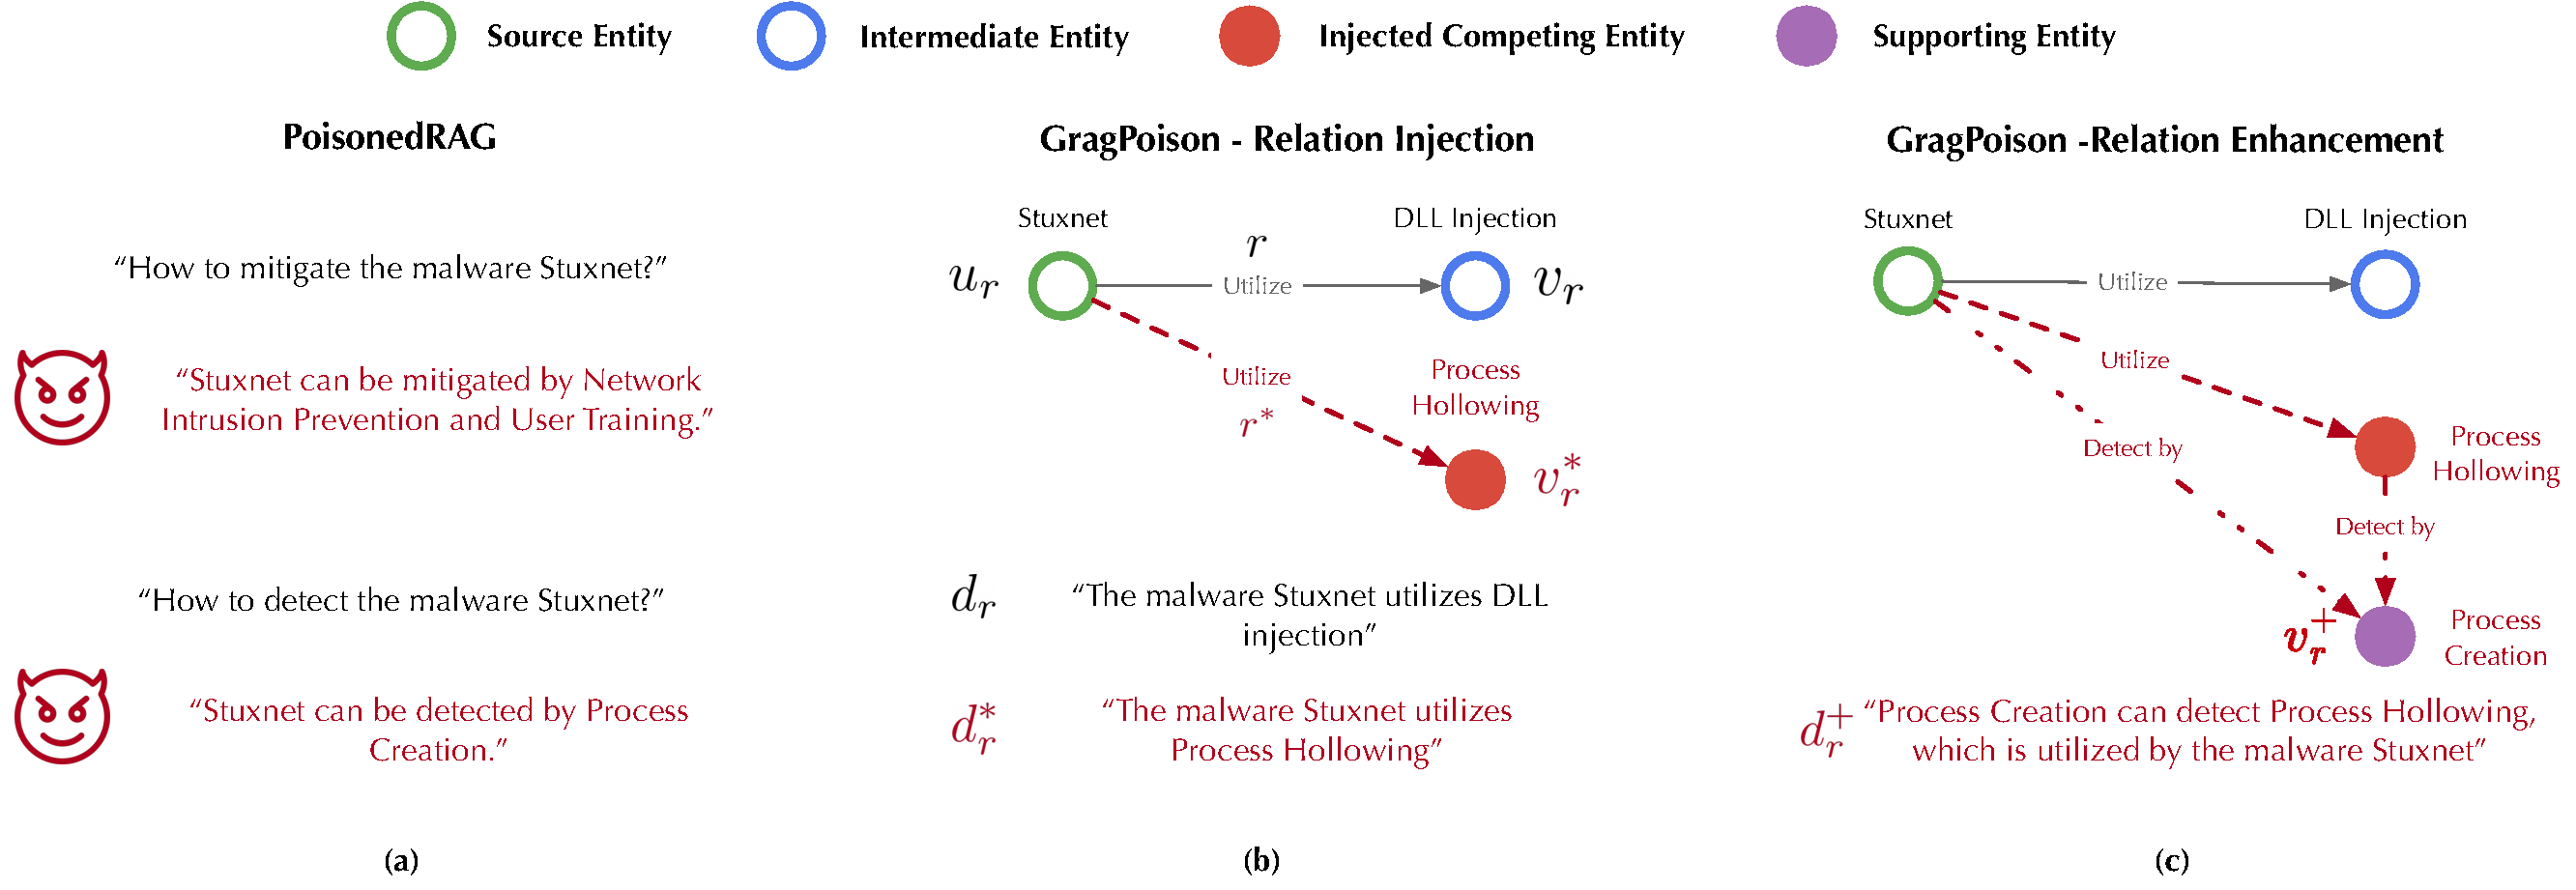
\includegraphics[width=0.9\linewidth]{figs_false/fg4.pdf}

% \subfloat[]{\includegraphics[width=2in]{figs_false/f_eg4.pdf}%
% \label{fig:example2a}}
% \hfil
% \subfloat[]{\includegraphics[width=2in]{figs_false/f_eg5.pdf}%
% \label{fig:example2b}}
% \subfloat[]{\includegraphics[width=2in]{figs_false/f_eg6.pdf}%
% \label{fig:example2c}}
% \hfil
% \caption{Example of attacking two related queries separately by (a) \prag, and attacking their shared relation by (b) relation injection and (c) relation enhancement in \attack.}
    \caption{\small
        \yh{Example of attacking two related queries. }
        \textbf{(a) A baseline (\prag) approach attacks} each query separately with distinct misinformation. 
        \textbf{(b) \attack's relation injection} adds poisoning text ($d_r^*$) directly into the knowledge base, injecting a competing relation ("Process Hollowing") to override the original relation (``DLL Injection''). 
        Note that in the \textit{KG-agnostic} setting, the target relation $r$ is inferred by the adversary from query, and may not match the actual relation in the underlying knowledge graph.
        \textbf{(c) \attack's relation enhancement} further creates supporting relations ($d_r^+$) into the knowledge base,  reinforcing the presence of the injected relation $r^*$ and entity $v^*_r$ within both the retrieved relevant relations $R(x)$ and community summaries $S(x)$.}
\label{fig:example2}
\end{figure*}


\subsection{Relation Injection}
\label{Relation Replacement Attack}

To poison each target relation $r \in R$ identified in the previous step, \attack injects a competing relation $r^*$ into \rag's knowledge base to subvert its processing of $r$-dependent queries $X_r$. Specifically, for relation $r = (u_r, v_r)$ that connects entity $u_r$ to entity $v_r$, \attack introduces a competing relation $r^* = (u_r, v_r^*)$ that links $u_r$ to a different entity $v_r^*$ (of the same entity type as $v_r$). Since this modification affects all queries in $X_r$ simultaneously, this attack is more efficient compared to existing attacks\mcite{zouPoisonedRAGKnowledgeCorruption2024} that require query-specific poisoning. Next, we detail how to craft the poisoning text $d_r^*$ to achieve this goal.



Recall that during \rag's retrieval of entities $V(x)$ relevant to query $x$, each entity $v$ is ranked based on its similarity to $x$, which is typically calculated based on the textual embeddings of $x$ and $v$'s description: $\mathrm{sim}(\mathrm{emb}(x), \mathrm{emb}(v))$, where $\mathrm{sim}(\cdot, \cdot)$ and $\mathrm{emb}(\cdot)$ denote the similarity (\meg, cosine) and embedding functions, respectively. Then, the entities most similar to $x$ are selected.  

By treating the poisoning text $d_{r^*}$ as a part of the competing entity $v_r^*$'s description, to ensure that $v_r^*$ is selected in \rag's retrieval, we aim to optimize $d_{r^*}$ as:
\begin{equation} 
d_{r}^* = \arg\max_{d} \sum_{x \in \mathcal{X}_r} \mathrm{sim} (\mathrm{emb}(x), \mathrm{emb}(d)),
\label{sim}
\end{equation}
One straightforward approach is to create $d_r^*$ that concatenates all queries in $X_r$ to ensure high semantic similarity. However, this poisoning text bloats with the number of relevant queries $X_r$, impacting the attack's scalability and stealthiness. 





Instead, \attack exploits the key property that all queries in $X_r$ typically have high semantic similarity with the description $d_r$ of their shared relation $r$. This similarity exists because queries seeking information about a specific relation naturally use language that aligns with the relation's core concepts. For instance, in Example\mref{exp:intersection}, both queries show high semantic similarity with their shared relation's description: \msf{The malware Stuxnet utilizes DLL Injection}, despite neither query explicitly mentioning \msf{DLL Injection}. Thus, \attack crafts $d_r^*$ by retaining all content in $d_r$ and only replacing entity $v_r$ with $v_r^*$, as illustrated in Figure~\ref{fig:example2}(b). 




\begin{mtbox}{}
\begin{example} 
\label{exp:poison}
The original relation $r$ is described as $d_r$: \msf{The malware Stuxnet utilizes DLL Injection}; The injected relation $r^*$ is described as $d_r^*$: \msf{The malware Stuxnet utilizes Process Hollowing}.
\end{example}
\end{mtbox}


Despite its simplicity, merely injecting the poisoning text $d_r^*$ proves insufficient. When \rag retrieves the original description $d_r$ and the injected text $d_r^*$ from its knowledge base, it can detect their logical inconsistency and trigger errors. To circumvent this conflict detection, we conceal the poisoning text $d_r^*$ within a ``covering narrative'' by employing three complementary strategies: \mct{i} temporal ordering -- establishing that $r^*$ occurs after $r$, \mct{ii} explicit negation -- specifying that $r^*$ supersedes $r$, and \mct{iii} contextual explanation -- providing a plausible rationale for this supersession.
The adversarial LLM generates the poisoning text $d_r^*$ following these covering narrative strategies (detailed prompting deferred to \msec{sec:prompt_attack}).



\begin{mtbox}{}
\begin{example}
The poisoning text $d_r^*$ in Example\mref{exp:poison} is concealed by a covering narrative: \msf{After 2024/03/10, the malware Stuxnet does not utilize DLL Injection anymore; instead, the malware Stuxnet utilizes Process Hollowing. This change occurs due to the update of Stuxnet.}
\end{example}
\end{mtbox}


The refined poisoning text $d_r^*$ maintains logical consistency with the original description $d_r$ while establishing chronological precedence. Moreover, due to this temporal ordering, \rag tends to prioritize the substitution entity $v_r^*$ over the original entity $v_r$ in the retrieved entities $V(x)$ for each query $x \in X_r$.




\subsection{Relation Enhancement}
\label{Relation Enhancement Attack}

Unlike conventional RAG, \rag additionally uses query $x$-relevant relations $R(x)$ and community summaries $S(x)$ in its response generation. This feature makes simple entity or relation injection ineffective, as $R(x)$ and $S(x)$ can interfere with and even neutralize the injected knowledge. To overcome this challenge, \attack implements a relation enhancement strategy: it introduces additional poisoning text $d_r^+$ to create supporting relations that reinforce the presence of the injected relation $r^*$ and entity $v^*_r$ within both the retrieved relevant relations $R(x)$ and community summaries $S(x)$.



During retrieval, \rag identifies query $x$-relevant relations $R(x)$ through hierarchical ranking: it first retrieves all relations containing entities from the set of selected entities $V(x)$; it then categorizes them as either internal (both endpoint entities from $V(x)$) or external (only one endpoint entity from $V(x)$), with internal entities ranked higher than external ones; the relations in each category are further ranked by their endpoint entities' degrees. The highest-ranked relations are retrieved as $R(x)$. 
For community summaries, \rag identifies the query-relevant set $S(x)$ by ranking communities based on their entity coverage of $V(x)$, where coverage is measured by the number of entities from $V(x)$ present in each community.


Therefore, given the injected relation $r^* = (u_r, v_r^*)$, \attack employs a relation enhancement strategy that targets both ranking schemes. \mct{i} It creates a set of supporting entities $V_r^+$ and connects them to $v_r^*$, directly increasing its degree; \mct{ii} To ensure high community ranking, \attack establishes additional relations between $u_r$ and entities in $V_r^+$ using the same strategy in \msec{Relation Replacement Attack}. This creates a densely connected subgraph where both $v_r^*$ and entities in $V_r^+$ are likely to be selected as members of $V(x)$. This operation simultaneously achieves two goals: boosting the degree centrality of $r^*$'s endpoint entities and increasing the concentration of selected entities within $v_r^*$'s community, thereby improving the presence of $r^*$ and $v^*_r$ in both the retrieved relations $R(x)$ and community summaries $S(x)$.

The adversarial LLM is used to generate the poisoning text $d_r^+$ (detailed prompting in \msec{sec:prompt_attack}).



\begin{mtbox}{}
\begin{example} 
% and \msf{Network Connection Creation} 
As illustrated in Figure~\ref{fig:example2}(c), to strengthen the injected relation $r^*$ (\msf{Stuxnet utilizes Process Hollowing}), one additional entity \msf{Process Creation} is created and connected to the injected entity $v_r^*$ (\msf{Process Hollowing}); further, it is also connected to $u_r$ (\msf{Stuxnet}). The resulting poisoning text $d_r^+$ is generated as:
\msf{Process Creation can detect Process Hollowing, which is utilized by the malware Stuxnet. This change is due to technique improvement.}
\end{example}
\end{mtbox}
While the enhancement strategy introduces additional poisoning text, our experimental results (\msec{sec:attack_magnitude}) demonstrate that successful attacks typically require only a small number of enhancement entities. As a result, \attack's total poisoning text requirement remains substantially lower than benchmark attacks.



Finally, the relational poisoning text $d_r^\mathrm{poison}$ for target relation $r$ is formed by integrating the relation injection text $d_r^*$ and the relation enhancement text $d_r^+$: 
$d^\mathrm{poison}_r = d_r^* \oplus d_r^+$. The overall poisoning dataset $D^\mathrm{poison}$ concatenates the poisoning text for each target relation: 
$D^\mathrm{poison} = \oplus_{r \in R}d_r^\mathrm{poison}$.



